\documentclass{article}
\usepackage[T1]{fontenc}

\usepackage{graphicx}
\usepackage{listings}
\begin{document}

\title{FOSS Lab Report}
\author{Gokul K\\[2\baselineskip]
Roll Number: 21\\[2\baselineskip]}
\date{02 February 2020}

\maketitle

\setcounter{section}{14}
\section{Shell Programming XI}
\subsection{Aim}
Write a shell script that will take an input file and remove identical lines


\subsection{Source Code}
\begin{verbatim}
    #! /bin/bash

    # Gokul K
    # Roll No: 21
    # 25-01-2020

    # Write a shell script that will take an input file and remove identical lines

    if [[ $# -ne 1 || !(-f $1) ]]
    then
        echo "Enter filename"
        exit
    fi

    text="`sort $1 | uniq`"
    echo "$text" > $1

\end{verbatim}

\subsection{Program Description}
Filename is provided as an argument, hence refered as \$1. uniq is an UNIX command
which outputs only unique lines from a sorted input. Hence the content of file is
sorted before piping to uniq. The output is then redirected to the original file

\subsection{Output}
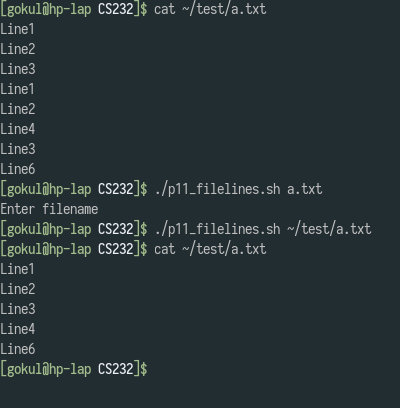
\includegraphics[width=0.9\textwidth]{img/p15.png}\newline

\subsection{Result}
The above program is run on Manjaro Linux shell. The unique lines in the
file is obtained as output
\end{document}